% vim: ts=2:sw=2:tw=80:et
\thispagestyle{fancy}
\pagestyle{fancy}

\section{Waveform Basics}

\begin{figure}[ht]
  \centerline{a)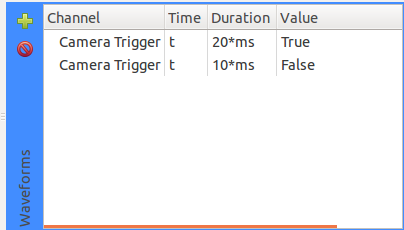
\includegraphics[width=.5\textwidth]{figures/waveform-0}}
  \centerline{b)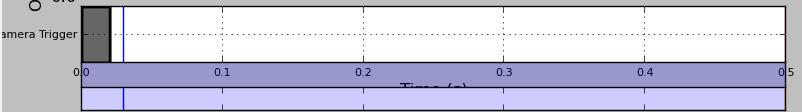
\includegraphics[width=.8\textwidth]{figures/plot-0}}
  \caption[Very simple waveform]{
    a) Add some simple waveform elements.
    b) Plot of simple waveform elements.
  }
  \label{fig:quick:waveform-0}
\end{figure}

\begin{figure}[ht]
  \centerline{a)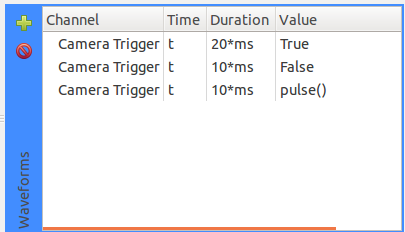
\includegraphics[width=.5\textwidth]{figures/waveform-1}}
  \centerline{b)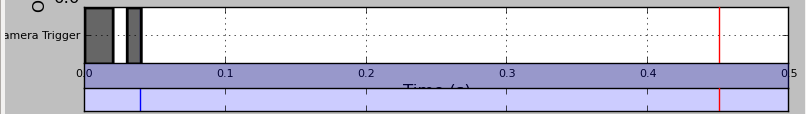
\includegraphics[width=.8\textwidth]{figures/plot-1}}
  \caption{a) Add some simple waveform elements. b) Plot of simple
  waveform elements.}
  \label{fig:quick:waveform-1}
\end{figure}

\begin{figure}[ht]
  \centerline{a)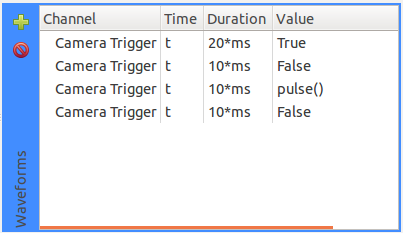
\includegraphics[width=.5\textwidth]{figures/waveform-2}}
  \centerline{b)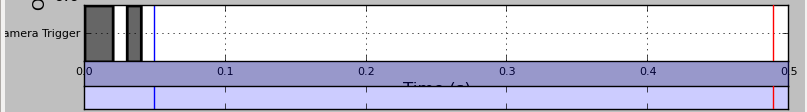
\includegraphics[width=.8\textwidth]{figures/plot-2}}
  \caption{a) Add some simple waveform elements. b) Plot of simple
  waveform elements.}
  \label{fig:quick:waveform-2}
\end{figure}

\begin{figure}[ht]
  \centerline{a)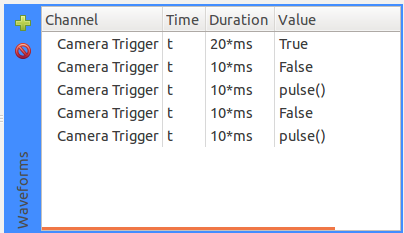
\includegraphics[width=.5\textwidth]{figures/waveform-3}}
  \centerline{b)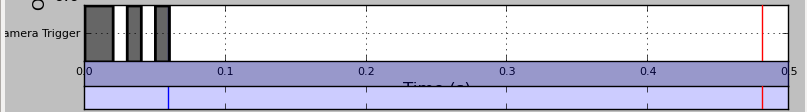
\includegraphics[width=.8\textwidth]{figures/plot-3}}
  \caption{a) Add some simple waveform elements. b) Plot of simple
  waveform elements.}
  \label{fig:quick:waveform-3}
\end{figure}


\subsection{Natural Time and Duration}

\begin{table}
\begin{center}
  \begin{tabular}{|l | c | c | c |}
    \hline
    Variable Name  & Description  & Group Scope & Waveform Element Scope \\
    \hline
    \symb{natural_time} & Currently progressed natural time & X & X \\
    \symb{duration}     & Duration of current group & X & X \\
    \symb{dt_clk}       & Minimum clock period of channel &  & X \\
    \symb{U0}           & Last value of channel &  & X \\
    \symb{relative_time}& Relative waveform-element time &  & X \\
   \hline
  \end{tabular}
  \caption[Automatic waveform variables]{
    Automatically defined waveform variables allow natural and easy entry of
    waveform elements.
  }
\end{center}
\end{table}


\section{Groups}

\begin{figure}[ht]
  \centerline{a)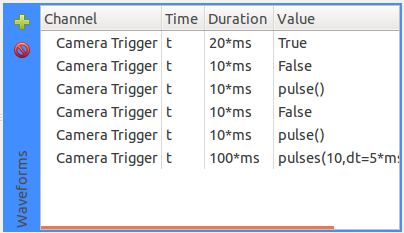
\includegraphics[width=.5\textwidth]{figures/waveform-4}}
  \centerline{b)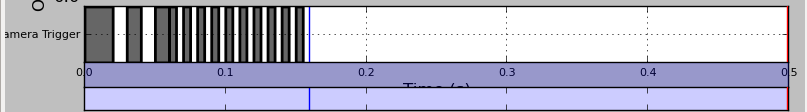
\includegraphics[width=.8\textwidth]{figures/plot-4}}
  \caption{a) Add some simple waveform elements. b) Plot of simple
  waveform elements.}
  \label{fig:quick:waveform-4}
\end{figure}

\begin{figure}[ht]
  \centerline{a)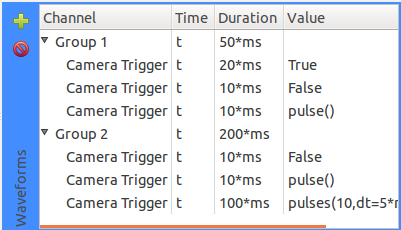
\includegraphics[width=.5\textwidth]{figures/waveform-5}}
  \centerline{b)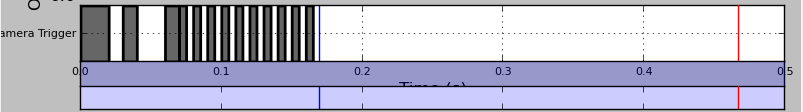
\includegraphics[width=.8\textwidth]{figures/plot-5}}
  \caption{a) Waveform elements divided into two main groups. b) Plot of
  waveform after grouping elements.}
  \label{fig:quick:waveform-5}
\end{figure}

\begin{figure}[ht]
  \centerline{a)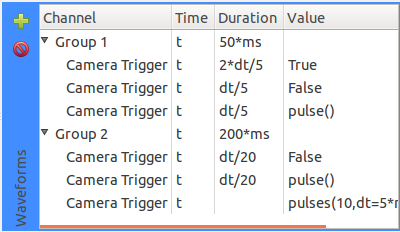
\includegraphics[width=.5\textwidth]{figures/waveform-6}}
  \centerline{b)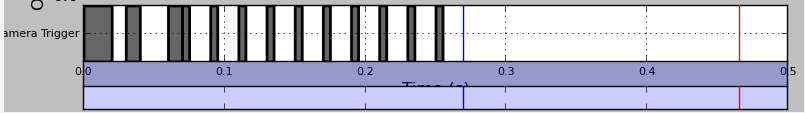
\includegraphics[width=.8\textwidth]{figures/plot-6}}
  \caption{a) Using automatic $dt$ variable. b) Plot of waveform after
  using $dt$ variable.}
  \label{fig:quick:waveform-6}
\end{figure}

\subsection{Subgroups}


\section{Waveform Elements}
\subsection{Value Expressions}
\subsubsection{Basics}
The value of each waveform element, in the most basic form, may be specified as
a single value with units appropriate for the respective channel.

Often times, a single value for a waveform element is not sufficient.  Arbwave
provides two mechanisms that allow a single waveform element to represent a
time-varying function.  The simplest of these two is using \textit{Value
Expressions}, as described in here.  The second mechanism is using the much more
powerful, extensible, but much more complicated-to-extend \textit{Value
Generators }--see help menu for more information.

If the sympy package is available, Arbwave uses it to allow the user to specify
functional forms of values for a waveform element.  When using expressions, in
order to define how a channel's value should change over time, one uses the
symbol \symb{relative_time} to represent relative waveform-element time.
\symb{relative_time} always varies
from 0 to 1.  Thus, for a waveform element with duration \symb{duration},
\symb{relative_time} varies from 0 to 1
over the duration of the waveform element.

As an example of using expressions, consider the \op{Ramp} value generator
function.  This function generally varies the channel as:
%
\begin{lstlisting}
  U0 + (U1 - U0)*x**E
\end{lstlisting}
%
where U0 and U1 are the beginning and ending values of the ramp respectively and
E is the power of the time dependence.  If, for instance, a voltage channel
required to be changed from its original value to a final value of 10*V with a
square-root time dependence, one could simply use an expression like:
%
\begin{lstlisting}
  U0 + (10*V - U0)*x**0.5
\end{lstlisting}
%
Using expressions, it is much simpler for the user to specify somewhat arbitrary
functional forms of waveform values.  For instance, one can specify an Gaussian
change function as something like:
%
\begin{lstlisting}
  10*V * sy.exp(-(x-.5)**2.0 / (2 * .1**2.0))
\end{lstlisting}
%
where sy represents the sympy module as imported in the global script as:
\begin{lstlisting}
  import sympy as sy
\end{lstlisting}

\subsubsection{Value Expressions Advanced}
Just as many \textit{Value Generators} allow the user to use functional arguments to
modify the waveform generated, such as the number of steps in a \op{Ramp},
\textit{Value Expressions} similarly provides a method to modify the output.
%
There are three primary parameters to modify the resulting waveform of an
expression:
\begin{itemize}
  \item \var{expr\_fmt}
    \begin{itemize}
    \item uniform\\
      Causes the output waveform to be uniformly discretized in time.
    \item optimize\\
      Causes the output waveform to be optimally discretized in time such that a
      constant total err (\var{expr\_err}) is maintained for each linear
      time segment.
    \end{itemize}
  \item \var{expr\_steps}
      For \op{expr\_fmt = uniform}, this sets the number of fixed-size steps
      to make over the duration.
      For \op{expr\_fmt = optimize}, \op{1/expr\_steps} defines the
      minimal relative time-step to consider when creating a line segment that
      maximally incurs a total error equal to \var{expr\_err}.
  \item \var{expr\_err}
      See "optimize" above.
\end{itemize}
%
There are three possible methods to set each of these \textit{Value Expression}
parameters:
\begin{itemize}
  \item globally (i.e. in embedded Python shell or in global script)
  \item local to group (in a local group script)
  \item local to waveform element:\\
    If one desires the scope of these parameters to be limited to a single
    element, one must wrap the expression by the \op{expr} function.
    The signature to this function is given by:\\
      \op{expr(expression, steps=None, err=None, fmt=None)}
\end{itemize}



\subsection{Value Generators}
Value generators allow more power waveform generation control for a single
waveform element.  Rather than simply expressing the functional form of the
waveform element, a value generator instantiates the respective value-generator
class, which is then responsible for returning an iterator of waveform points
back to arbwave.
%
\begin{lstlisting}
class ValueGenerator(object):
  # Arbwave uses this string to represent the generator to the user.  It must be
  # a valid Python identifier, but may be something different than the exact
  # spelling (including case) of the generator class.
  name = 'valueGenerator'

  def __init__(self, arg0, arg1, arg2):
    """
    Usage:  valueGenerator(arg0, arg1, arg2)

    When the user creates the generator using the Python identifier from
    self.name, this is the constructor called (i.e. the signature of the
    generator).  The various arguments depend on the generator's use and may
    include default values.

    ***The documentation provided here is shown to the user in the \textit{Value
    Generators} help menu.***
    """
    super(ValueGenerator, self).__init__()
    ...

  def set_vars(self, _from, t, duration, dt_clk):
    """
    Arbwave uses this function to give channel-specific information to the
    generator.
      _from : is the last value (with units) of this channel before this
              waveform element
      t     : is the absolute start time of the waveform element ***in integer
              units of dt_clk***
      dt    : is the duration of the waveform element ***in integer units of
              dt_clk***
      dt_clk: is the duration of the clock pulse that is used for this channel
              in proper units (seconds)
    """
    pass

  def set_units(self, units, units_str):
    """
    Arbwave calls this function if it exists to give the generator the
    user-specified units and units string for the particular channel.
    """
    pass

  def get_encoding(self, capabilities):
    """
    Given the set of capabilities supported by the channel, this function
    returns the encoding desired.
    """
    pass

  def __repr__(self):
    """
    Show return a string that correctly represents the constructor of the
    generator as used by the user.  This will be used in tooltips to show the
    value of the waveform element.
    """
    pass

  def __iter__(self):
    """
    Must return an iterator that runs over the generated waveform.

    Each value returned by this iterator must be a tuple such as:
    (t, dt, v)
    where t and dt are the start time and duration of the waveform component
    ***in units of dt_clk*** for the channel respectively and v is the value
    (with the correct units for the channel).
    """
    pass

\end{lstlisting}
%
Currently, several value generators are supplied directly by Arbwave:
\begin{itemize}

\item \op{sinpulse}
\begin{lstlisting}
"""
    Usage:  sinpulse(A, F, average=0., phase_shift=0., steps_per_cycle=None):

    A       : Amplitude (0-to-peak)
    F       : Frequency in Hz
    average : Average value of sine wave.
    phase_shift : 0 to 2 pi shift, where pi/2 represents +cos
    steps_per_cycle   : number of steps per cycle

    Only one of dt or steps can be used.
"""
\end{lstlisting}

\item \op{ramp}
\begin{lstlisting}
"""
Usage:  ramp(to, exponent=1.0, steps=20, _from=None, dt=None, duration=None)

to      : final value to which to ramp
_from   : initial value from which to ramp
exponent: exponent with which to ramp
steps   : number of steps to take
dt      : the timestep to increment (Default: duration/steps)
duration: Duration of ramp function.  Note that this is not necessarily
          equal to the actual duration of the steps generated by the ramp,
          since those are set in the "Duration" field of the waveform
          editor.  Value of None indicates that the ramp should last for the
          time specified in the "Duration" field of the waveform editor.
          [Default: None]

Only one of dt or steps can be used.
"""
\end{lstlisting}

\item \op{pulse}
\begin{lstlisting}
"""
Usage:  pulse(high=True, low=None)

high  : The value to generate for the pulse.
low   : The value to return to after the pulse.
        If low is not set (left as None) it will be set differently for
        analog and digital channels.  If the high is a boolean value, low
        will be set to its logical complement.  Otherwise, if low is not
        set, it will be set to whatever the channel is at prior to this
        pulse.
"""
\end{lstlisting}

\item \op{pulses}
\begin{lstlisting}
"""
Usage:  pulses(n, duty=0.5, high=True, low=False, dt=None)

n     : Number of evenly spaced pulses to generate.
duty  : Duty cycle (only used if dt is not set) [Default 0.5].
high  : The value to generate for each pulses [Default:  True].
low   : The value to return to after the pulse.
        If low is not set (left as None) it will be set differently for
        analog and digital channels.  If the high is a boolean value, low
        will be set to its logical complement.  Otherwise, if low is not
        set, it will be set to whatever the channel is at prior to this
        pulse.
"""
\end{lstlisting}

\item \op{interp}
\begin{lstlisting}
"""
Usage:  interp(x, y, steps=20, dt=None)

x       : time in arbitrary units.  Time will be normalized to 0-1 where
          time=1 corresponds to the maximum value in x.
y       : y values to use in interpolation
steps   : number of steps to take (Default: 20)
dt      : the timestep to increment (Default: duration/steps)

Only one of dt or steps can be used.
"""
\end{lstlisting}

\end{itemize}
